\documentclass[a4paper]{article}
%\documentclass[a4paper,10pt]{scrartcl}

\usepackage[utf8]{inputenc}
\usepackage[margin=0.9in]{geometry}
\usepackage{pgf}
\usepackage{tikz}
\usepackage{float}
\usepackage{stmaryrd}
\usetikzlibrary{arrows}
\usetikzlibrary{automata}
\definecolor{lgrey}{RGB}{190,190,190}
\pdfinfo{%
  /Title    (Assessed Coursework: Systems Verification 303)
  /Author   (Ioannis Kassinopoulos)
  /Creator  (Ioannis Kassinopoulos)
  /Producer (Ioannis Kassinopoulos)
  /Subject  (Systems Verification Coursework)
  /Keywords (verification,coursework,imperial)
}

\begin{document}

\title{Assessed Coursework: Systems Verification}
\author{Ioannis Kassinopoulos}
\date{\today}
\maketitle
\section*{Question 1}
\begin{figure}[H]
  \centering
  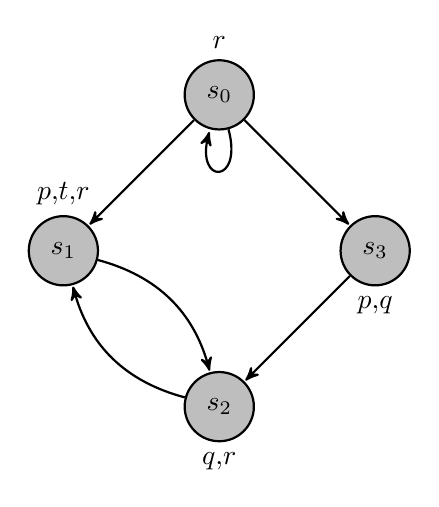
\begin{tikzpicture}[->,>=stealth',shorten >=0.5pt,auto,node distance=2.8cm,thick]
      \tikzstyle{every state}=[fill=lgrey,draw=black,text=black]

      \node[label = above:{$r$},state]		(A) {$s_0$};
      \node[label = above:{$p$,$t$,$r$},state]	(B) [below left of  = A]   {$s_1$};
      \node[label = below:{$p$,$q$},state]	(C) [below right of = A]   {$s_3$};
      \node[label = below:{$q$,$r$},state]	(D) [below right of = B]   {$s_2$};
      
      \path 
	(A) edge			node{} (B)
	(A) edge			node{} (C)
	(A) edge	[loop below]	node{} (A)
	(B) edge	[bend left]	node{} (D)
	(D) edge	[bend left]	node{} (B)
	(C) edge			node{} (D);
      
  \end{tikzpicture}
  \caption{The transition system $\mathcal{M}_1$.}
  \label{fig:m1}
\end{figure}

\subsection*{Algebraic Form}

A transition system $\mathcal{M}=(S,\rightarrow,\pi)$ is a set of states $S$ endowed with a transition relation 
$\rightarrow$ (a binary relation on $S$), such that every $s \in  S$ has some $s'\in S$ with $s\rightarrow s'$,
and an inverse labeling function $\pi:\mathcal{P}\rightarrow S$.
\\[0.5cm] 
Our system $\mathcal{M}_1$ (figure:~\ref{fig:m1}) can be described as following:
\\[0.cm] 
$\mathcal{P} = \{p,q,r,t\}$
\\[0.10cm] 
$\mathcal{M}_1 = \{\{ s_0,s_1,s_2,s_3 \} , \{ (s_0,s_0),(s_0,s_1),(s_0,s_3),(s_1,s_2),(s_2,s_1),(s_3,s_2)   \} , \pi \}$
\\[0.10cm] 
$\pi(p) = \{s_1,s_3 \}$
\\[0.10cm] 
$\pi(q) = \{s_2,s_3 \}$
\\[0.10cm] 
$\pi(r) = \{s_0,s_1,s_2 \}$
\\[0.10cm] 
$\pi(t) = \{ s_1 \}$
\subsection*{Infinite Tree}
\begin{figure}[H]
  \label{fig:infTree}
  \centering
  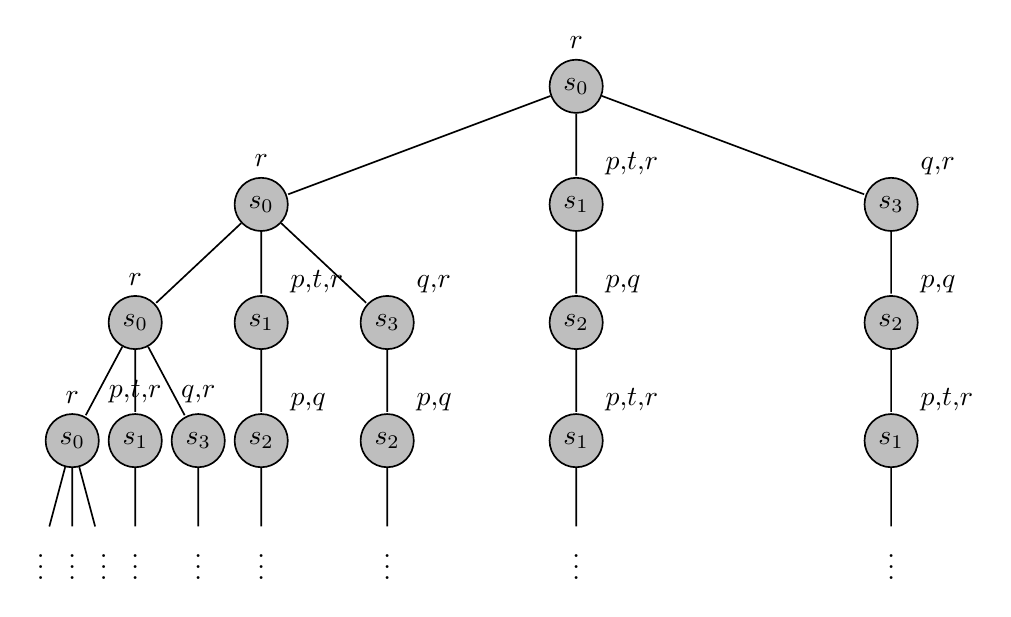
\begin{tikzpicture}[level 2/.style={sibling distance=16mm},level 1/.style={sibling distance=40mm},level 4/.style={sibling distance=4mm},level 3/.style={sibling distance=8mm},level/.style={sibling distance=25mm/#1},-,>=stealth',shorten >=0.5pt,auto,node distance=1cm,semithick]
      \tikzstyle{every state}=[fill=lgrey,draw=black,text=black,inner sep=3pt,minimum size=4pt]
      \node [label = above:{$r$},state] (a){$s_0$}
	child {
	node [label = above:{$r$},state] (b) {$s_0$}
	  child {
	  node [label = above:{$r$},state] (c) {$s_0$}
	    child{
	    node [label = above:{$r$},state] (d) {$s_0$}
	      child{
	      node [] (e) {$\vdots$}
	      }
	      child{
	      node [] (e) {$\vdots$}
	      }
	      child{
	      node [] (e) {$\vdots$}
	      }
	    }
	    child{
	    node [label = above:{$p$,$t$,$r$},state] (d) {$s_1$}
	      child{
	      node [] (e) {$\vdots$}
	      }
	    }
	    child{
	    node [label = above:{$q$,$r$},state] (d) {$s_3$}
	    child{
	      node [] (e) {$\vdots$}
	      }
	    }
	  }
	  child {
	  node [label = above right:{$p$,$t$,$r$},state] (c) {$s_1$}
	    child {
	    node [label = above right:{$p$,$q$},state] (d) {$s_2$}	      
	    child {
	    node [] (e) {$\vdots$}	      
	    }
	    }
	  }	  
	  child {
	    node [label = above right:{$q$,$r$},state] (c) {$s_3$}
	      child {
	      node [label = above right:{$p$,$q$},state] (d) {$s_2$}	      
		child {
		node [] (e) {$\vdots$}	      
	      }
	    }
	  }
	}
	child {
	node [label = above right:{$p$,$t$,$r$},state] (b) {$s_1$}
	  child {
	  node [label = above right:{$p$,$q$},state] (c) {$s_2$}
	    child {
	    node [label = above right:{$p$,$t$,$r$},state] (d) {$s_1$}
	      child {
	      node [] (e) {$\vdots$}	      
	      }
	    }
	  }
	}
	child {
	node [label = above right:{$q$,$r$},state] (b) {$s_3$}
	child {
	node [label = above right:{$p$,$q$},state] (c) {$s_2$}
	  child {
	  node [label = above right:{$p$,$t$,$r$},state] (d) {$s_1$}
	    child {
	    node [] (e) {$\vdots$}
	    }
	  }
	}
	};
  \end{tikzpicture}
  \caption{Unwinding the system described by  $\mathcal{M}_1$ as an infinite tree of all computation paths beginning in $s_0$ (first layer).}
\end{figure}


\def\holds#1 #2 {$(\mathcal{M}_1,s_{#1})\models$ #2 }
\def\nholds#1 #2 {$(\mathcal{M}_1,s_{#1})\not\models$ #2 }
\def\pathr{$\rho = x_0,x_1,...=$ }



\subsection*{Satisfiability}
\subsubsection*{(a) LTL: $\phi = Ft$}
\nholds 0 $Ft$ 
\\[0.25cm]
since for path \pathr $s_0^+$   no state $x_i \not\in\pi(t)$ since $s_0$ $\not\in\pi(t)$
\\[0.50cm]
\holds 2 $Ft$
\\[0.25cm]
since the only path that exist is \pathr $(s_2,s_1)^+$ and for $x_i = s_1$ $\Rightarrow s_1 \in\pi(t)$
\subsubsection*{(b) CTL: $\phi = \neg EG r$}
$EGr =\neg AF\neg r \Rightarrow \neg EGr =\neg \neg AF\neg r= AF\neg r$ \\[0.25cm]
\nholds 0 $AF\neg r$ since for the path \pathr $s_0^+$ every state $x_i=s_0\in \pi(r)$ \\[0.25cm]
$\Rightarrow$ \nholds 0 $\neg EG r$ \\[0.25cm]
\nholds 2 $A\neg r$ since for the only path \pathr $(s_2,s_1)^+$ every state $x_i=s_1\in \pi(r)$ or $x_i=s_2\in \pi(r)$\\[0.25cm]
$\Rightarrow$ \nholds 2 $\neg EG r$ 


\subsubsection*{(c) CTL: $\phi = E(tUq)$}
\nholds 0 $E(tUq)$ 
\\[0.25cm]
since for every (and therefore for at least one) path \pathr $s_0,...$ at $s_0$, $s_0 \not\in \pi(t) \cup \pi(q)$.
\\[0.25cm] therefore, since at the initial state we have neither t nor q we cannot say that a path exists starting from $s_0$ such that t until q holds.
\\[0.50cm]
\holds 2 $E(tUq)$
\\[0.25cm]
since for the only path \pathr $(s_2,s_1)^+$ we have at $x_0 = s_2$, and \holds 2 $tUq$ since $s_2 \in \pi(q)$. This means that t is always true up to the point that q gets true.

\subsubsection*{(d) CTL*: $\phi = E(FGp)$}
For this formula we first need to consider all the possible tuples of transition relation given by the $\rightarrow$ set:
\\[0.25cm]
$ \{(s_0,s_0),(s_0,s_1),(s_0,s_3),(s_1,s_2),(s_2,s_1),(s_3,s_2) \}$ 
\\[0.50cm]
As we can see from the $\pi(p)$ set, no two concequtive states $x_i,x_{i+1} \in \pi(p)$ which means that for every state $s_i$: \nholds i $Gp$, \nholds i $FGp$
and  \nholds i $E(FGp)$ \\[0.25cm]
Therefore we can say that: \\[0.25cm]
\nholds 0 $E(FGp)$
\\[0.25cm]
\nholds 2 $E(FGp)$
\\[0.25cm]
since no path exists which eventually gets forever p starting from either $s_0$ or $s_2$

\subsubsection*{(e) CTL: $\phi = EGr$}
$ EGr = \neg \neg EGr $ therefore from the $\phi = \neg EGr$ solution we can deduce that:\\[0.25cm]
\holds 0 $EGr$ since \nholds 0 $\neg EGr\:$ since $true = \neg false$
\\[0.25cm]
and
\\[0.25cm]
\holds 2 $EGr$ since \nholds 2 $\neg EGr$  since $true = \neg false$
\subsubsection*{(f) LTL: $\phi = G(r \vee q)$}
From the model we can see that the following are true:
\\[0.25cm]
$s_0 \in \pi(r) \cup \pi(q) $ since $s_0 \in \pi(r)$ so \holds 0 $r \vee q$
\\[0.25cm]
$s_1 \in \pi(r) \cup \pi(q) $ since $s_1 \in \pi(r)$ so \holds 1 $r \vee q$
\\[0.25cm]
$s_2 \in \pi(r) \cup \pi(q) $ since $s_2 \in \pi(q)$ so \holds 2 $r \vee q$
\\[0.25cm]
$s_3 \in \pi(r) \cup \pi(q) $ since $s_3 \in \pi(q)$ so \holds 3 $r \vee q$
\\[0.25cm]
We can therefore say that for every state $s_i$, \holds i $G(r \vee q)$ since every path, from every state, will satisfy $r \vee q$ forever (globally).
\\[0.25cm]
\holds 0 $G(r \vee q)$
\\[0.25cm]
\holds 2 $G(r \vee q)$
\subsubsection*{(g) LTL: $\phi = falseUp$}
\nholds 0 $falseUp$
since $s_0 \not\in \{ \} \cup \pi(p)$ therefore since the first state of the path does not fulfill p \\[0.25cm] $\Rightarrow$ false until p cannot be true.\\[0.25cm]
\nholds 2 $falseUp$
since $s_2 \not\in \{ \} \cup \pi(p)$ therefore since the first state of the path does not fulfill p \\[0.25cm] $\Rightarrow$ false until p cannot be true.
\subsubsection*{(h) CTL: $\phi = A(pU(EFq))$}
First, let's find which states satisfy $EFq$ \\[0.25cm]
$\{s_0,s_1,s_2,s_3\}$ satisfy $EFq$ since all of them are either labelled $q$ \\[0.25cm]
or have one of their next states satisfying $q$.\\[0.25cm]
This intuitively says for all  states $s_i$, \holds i $EFq$. \\[0.25cm]
This means that for all paths starting from every state of our model $pU(EFq)$ is true since we don't care about p being true since $EFq$ is always true at the first (initial) state. \\[0.25cm]
We can therefore deduce from the above that for all states $s_i$, \holds i  $A(pU(EFq))$ and: \\[0.25cm]
\holds 0 $A(pUEFq)$ \\[0.25cm]
\holds 2 $A(pUEFq)$

\newpage
\section*{Question 2}
\begin{figure}[H]
  \centering
  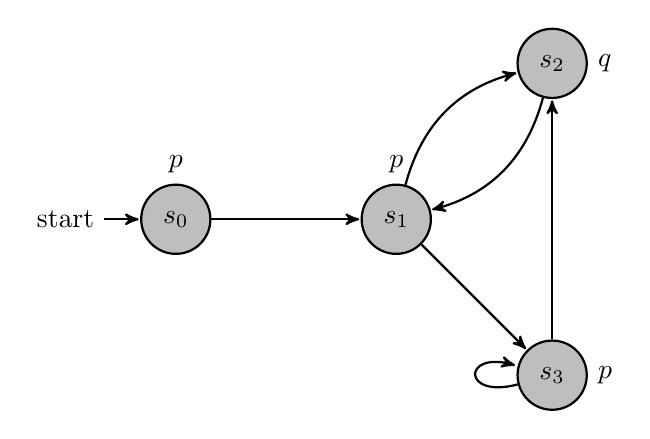
\begin{tikzpicture}[->,>=stealth',shorten >=0.5pt,auto,node distance=2.8cm,thick]
      \tikzstyle{every state}=[fill=lgrey,draw=black,text=black]

      \node[label = above:{$p$},initial,state]		(A) {$s_0$};
      \node[label = above:{$p$},state]		(B) [right of = A] {$s_1$};
      \node[label = right:{$q$},state]		(C) [above right of = B] {$s_2$};
      \node[label = right:{$p$},state]		(D) [below right of = B] {$s_3$};
      
      \path 
	(A) edge			node{} (B)
	(B) edge	[bend left]	node{} (C)
	(C) edge	[bend left]	node{} (B)
	(B) edge			node{} (D)
	(D) edge			node{} (C)
	(D) edge	[loop left]	node{} (D);
  \end{tikzpicture}
  \caption{The transition system $\mathcal{M}_2$.}
  \label{fig:m2}
\end{figure}

\subsection*{Calculating}

\subsection*{$\phi = p$}
\hspace*{5mm} $SAT(p)=\{ s \in S \mid p\in L(s)\} = \{s_0,s_1,s_3\}$ 
\\[0.25cm] 
\hspace*{5mm} $\Rightarrow \llbracket \phi \rrbracket = \{s_0,s_1,s_3\}$
\subsection*{$\phi = AGEFp$}
\hspace*{5mm} $SAT(EFp)=SAT(E[trueUp])=SAT_{eu}(true,p)$ 
\\[0.25cm] 
\hspace*{5mm}$SAT_{eu}(true,p)$ 
\\[0.25cm] 
\hspace*{10mm} $W = \{s_0,s_1,s_2,s_3\}$ 
\\[0.25cm] 
\hspace*{10mm} $Y_0 = \{s_0,s_1,s_3\}$ 
\\[0.25cm] 
\hspace*{10mm} $Y_1 = \{s_0,s_1,s_2,s_3\}$ 
\\[0.25cm] 
\hspace*{10mm} $Y_2 = Y_1$ 
\\[0.25cm] 
\hspace*{5mm} $SAT(AGEFp)=SAT(\neg EF \neg EF p)$ 
\\[0.25cm] 
\hspace*{5mm} $SAT(EF \neg EF p) =  SAT(E[trueU\neg EF p]) = SAT_{eu}(true,\neg EF p)$ 
\\[0.25cm] 
\hspace*{5mm} $SAT_{eu}(true,\neg EF p)$ 
\\[0.25cm] 
\hspace*{10mm} $W = \{s_0,s_1,s_2,s_3\}$ 
\\[0.25cm] 
\hspace*{10mm} $Y_0 = S \backslash \{s_0,s_1,s_2,s_3\} = \{ \}$ 
\\[0.25cm] 
\hspace*{10mm} $Y_1 = Y_0$ 
\\[0.25cm] 
\hspace*{4.9mm} $SAT(AGEFp)=SAT(\neg EF \neg EF p) = S\backslash SAT(EF \neg EF p) = \{s_0,s_1,s_2,s_3 \}$ 
\\[0.25cm] 
\hspace*{5mm} $\Rightarrow \llbracket \phi \rrbracket = \{s_0,s_1,s_2,s_3\}$

\subsection*{$\phi = AFq$}
\hspace*{5mm}$SAT(AFq) = SAT_{af}(q)$ 
\\[0.25cm] 
\hspace*{5mm}$SAT_{af}(q)$ 
\\[0.25cm] 
\hspace*{10mm}$Y_0 = \{s_2\}$
\\[0.25cm] 
\hspace*{10mm}$Y_1 = Y_0$ 
\\[0.25cm] 
\hspace*{5mm} $\Rightarrow \llbracket \phi \rrbracket = \{s_2\}$


\subsection*{$\phi = AGp \vee Afq$}
\hspace*{5mm}$SAT(AGp) = SAT(\neg EF \neg p)$ 
\\[0.25cm] 
\hspace*{5mm}$SAT(EF \neg p) = SAT(E[trueU \neg p]) = SAT_{eu}(true, \neg p)$ 
\\[0.25cm] 
\hspace*{5mm}$SAT_{eu}(true, \neg p)$ 
\\[0.25cm] 
\hspace*{10mm}$W = \{s_0,s_1,s_2,s_3\}$
\\[0.25cm] 
\hspace*{10mm}$Y_0 = S \backslash SAT(p) = \{s_2\}$
\\[0.25cm] 
\hspace*{10mm}$Y_1 = \{s_1,s_2,s_3\}$
\\[0.25cm] 
\hspace*{10mm}$Y_2 = \{s_0,s_1,s_2,s_3\}$
\\[0.25cm] 
\hspace*{10mm}$Y_3 = Y_2$
\\[0.25cm] 
\hspace*{5mm}$SAT(\neg EF \neg p) = S \backslash SAT( EF \neg p) = \{\}$ 
\\[0.25cm] 
\hspace*{5mm}$SAT(AGp \vee Afq) = SAT(AGp) \cup SAT(AFq) = \{\} \cup \{s_2\} = \{s_2\}$
\\[0.25cm] 
\hspace*{5mm} $\Rightarrow \llbracket \phi \rrbracket = \{s_2\}$

\subsection*{$\phi = E(pU(AFq))$}
\hspace*{5mm}$SAT(E[pU(AFq)]) = SAT_{eu}(p,AFq)$ 
\\[0.25cm] 
\hspace*{5mm}$SAT_{eu}(p,AFq)$ 
\\[0.25cm] 
\hspace*{10mm}$W = SAT(p) = \{s_0,s_1,s_3\}$
\\[0.25cm] 
\hspace*{10mm}$Y_0 = SAT(AFq) = \{s_2\}$
\\[0.25cm] 
\hspace*{10mm}$Y_1 = \{s_1,s_2,s_3\}$
\\[0.25cm] 
\hspace*{10mm}$Y_2 = \{s_0,s_1,s_2,s_3\}$
\\[0.25cm] 
\hspace*{10mm}$Y_3 = Y_2$
\\[0.25cm] 
\hspace*{5mm} $\Rightarrow \llbracket \phi \rrbracket = \{s_0,s_1,s_2,s_3\}$




\newpage
\section*{Question 3}
\subsection*{As one module}
\begin{verbatim}
MODULE main
VAR
	t1: {no_coal,has_coal,waiting,tunnel};
	t2: {no_coal,has_coal,waiting,tunnel};
	t3: {no_coal,has_coal,waiting,tunnel};
	cn: {0,1,2,3};
ASSIGN
	init(t1) := no_coal;
	next(t1) := 
		case
			t1 = no_coal: has_coal;
			t1 = has_coal: waiting;
			t1 = waiting & (cn=1): tunnel;
			t1 = waiting & !(cn=1): waiting;
			t1 = tunnel: no_coal;
		esac;

	init(t2) := no_coal;
	next(t2) := 
		case
			t2 = no_coal: has_coal;
			t2 = has_coal: waiting;
			t2 = waiting & (cn=2): tunnel;
			t2 = waiting & !(cn=2): waiting;
			t2 = tunnel: no_coal;
		esac;

	init(t3) := no_coal;
	next(t3) := 
		case
			t3 = no_coal: has_coal;
			t3 = has_coal: waiting;
			t3 = waiting & (cn=3): tunnel;
			t3 = waiting & !(cn=3): waiting;
			t3 = tunnel: no_coal;
		esac;
	init(cn) := 0;

	next(cn) := 
		case
			t1=waiting : 1;
			t2=waiting : 2;
			t3=waiting : 3;
			1: 0;
		esac;

SPEC
	AG(!(t1=tunnel & t2=tunnel & t3=tunnel))

SPEC
	AG(!(t1=tunnel) | AF(!(t1=tunnel)))

SPEC
	AG(!(t1=has_coal) | EF(!(t1=has_coal)))

SPEC
	AF(t1=tunnel)

\end{verbatim}
reachable states: 11 ($2^{3.45943}$) out of 256 ($2^8$)

\subsubsection*{CUDD statistics}
\begin{verbatim}

**** CUDD modifiable parameters ****
Hard limit for cache size: 2730666
Cache hit threshold for resizing: 30%
Garbage collection enabled: yes
Limit for fast unique table growth: 1638400
Maximum number of variables sifted per reordering: 1000
Maximum number of variable swaps per reordering: 2000000
Maximum growth while sifting a variable: 1.2
Dynamic reordering of BDDs enabled: no
Default BDD reordering method: 4
Dynamic reordering of ZDDs enabled: no
Default ZDD reordering method: 4
Realignment of ZDDs to BDDs enabled: no
Realignment of BDDs to ZDDs enabled: no
Dead nodes counted in triggering reordering: no
Group checking criterion: 7
Recombination threshold: 0
Symmetry violation threshold: 0
Arc violation threshold: 0
GA population size: 0
Number of crossovers for GA: 0
Next reordering threshold: 4004
**** CUDD non-modifiable parameters ****
Memory in use: 10544032
Peak number of nodes: 1022
Peak number of live nodes: 498
Number of BDD variables: 17
Number of ZDD variables: 0
Number of cache entries: 262144
Number of cache look-ups: 1047
Number of cache hits: 207
Number of cache insertions: 874
Number of cache collisions: 5
Number of cache deletions: 0
Cache used slots = 0.33% (expected 0.33%)
Soft limit for cache size: 18432
Number of buckets in unique table: 4608
Used buckets in unique table: 14.15% (expected 14.15%)
Number of BDD and ADD nodes: 722
Number of ZDD nodes: 0
Number of dead BDD and ADD nodes: 238
Number of dead ZDD nodes: 0
Number of LIVE BDD and ADD nodes: 484
Number of LIVE ZDD nodes: 0
Total number of nodes allocated: 722
Total number of nodes reclaimed: 190
Garbage collections so far: 0
Time for garbage collection: 0.00 sec
Reorderings so far: 0
Time for reordering: 0.00 sec 
\end{verbatim}

\subsection*{Modular}
\begin{verbatim}
MODULE train(signal,label)
VAR 
	state : {no_coal, has_coal, waiting, tunnel};
ASSIGN
 	init(state) := no_coal;
 	next(state) := 
 	case
 		(state = no_coal): has_coal;
 		(state = has_coal) : waiting;
 		(state = waiting) & (signal = label) : tunnel;
 		(state = tunnel) : no_coal;
 		1: state;
 	esac;

MODULE controller(t1, t2, t3)
VAR
  signal: {0,1,2,3};

ASSIGN
 init(signal):= 0;
 next(signal):=
	case
		t1.state = waiting : 1;
		t2.state = waiting : 2;
		t3.state = waiting : 3;
		1: 0;
	esac;

MODULE main 
 VAR
  	cn: controller(t1,t2,t3);
	t1: train(cn.signal,1);
 	t2: train(cn.signal,2);
 	t3: train(cn.signal,3);


 SPEC
  AG(!(t1.state=tunnel & t2.state=tunnel & t3.state=tunnel));
 SPEC
  AG(t1.state=tunnel -> AF!(t1.state=tunnel));
 SPEC
  AG(t1.state=has_coal -> EF !(t1.state=has_coal));
 SPEC
  AF(t1.state=tunnel);
 SPEC
  AG(EF(t1.state=tunnel));
\end{verbatim}
reachable states: 11 ($2^{3.45943}$) out of 256 ($2^8$)
\subsubsection*{CUDD statistics}
\begin{verbatim}
 **** CUDD modifiable parameters ****
Hard limit for cache size: 2730666
Cache hit threshold for resizing: 30%
Garbage collection enabled: yes
Limit for fast unique table growth: 1638400
Maximum number of variables sifted per reordering: 1000
Maximum number of variable swaps per reordering: 2000000
Maximum growth while sifting a variable: 1.2
Dynamic reordering of BDDs enabled: no
Default BDD reordering method: 4
Dynamic reordering of ZDDs enabled: no
Default ZDD reordering method: 4
Realignment of ZDDs to BDDs enabled: no
Realignment of BDDs to ZDDs enabled: no
Dead nodes counted in triggering reordering: no
Group checking criterion: 7
Recombination threshold: 0
Symmetry violation threshold: 0
Arc violation threshold: 0
GA population size: 0
Number of crossovers for GA: 0
Next reordering threshold: 4004
**** CUDD non-modifiable parameters ****
Memory in use: 10544032
Peak number of nodes: 1022
Peak number of live nodes: 491
Number of BDD variables: 17
Number of ZDD variables: 0
Number of cache entries: 262144
Number of cache look-ups: 888
Number of cache hits: 243
Number of cache insertions: 680
Number of cache collisions: 3
Number of cache deletions: 0
Cache used slots = 0.26% (expected 0.26%)
Soft limit for cache size: 18432
Number of buckets in unique table: 4608
Used buckets in unique table: 12.15% (expected 12.59%)
Number of BDD and ADD nodes: 635
Number of ZDD nodes: 0
Number of dead BDD and ADD nodes: 168
Number of dead ZDD nodes: 0
Number of LIVE BDD and ADD nodes: 467
Number of LIVE ZDD nodes: 0
Total number of nodes allocated: 635
Total number of nodes reclaimed: 137
Garbage collections so far: 0
Time for garbage collection: 0.00 sec
Reorderings so far: 0
Time for reordering: 0.00 sec


\end{verbatim}

  \newpage
\section*{Question 4}
Let $\phi = (x_1 \wedge x_2) \vee (y_1 \wedge y_2) $, the following truth table is derived to help us with our calculations

\begin{center}
 
\begin{tabular}{|c|c|c|c|c|c|c|}
\hline
$x_1$ & $x_2$ & $y_1$ & $y_2$ & $x_1 \wedge x_2 $ & $y_1 \wedge y_2$ & $(x_1 \wedge x_2) \vee (y_1 \wedge y_2)$ \\
\hline
0 & 0 & 0 & 0 & 0 & 0 & 0 \\
0 & 0 & 0 & 1 & 0 & 0 & 0 \\
0 & 0 & 1 & 0 & 0 & 0 & 0 \\
0 & 0 & 1 & 1 & 0 & 1 & 1 \\
0 & 1 & 0 & 0 & 0 & 0 & 0 \\
0 & 1 & 0 & 1 & 0 & 0 & 0 \\
0 & 1 & 1 & 0 & 0 & 0 & 0 \\
0 & 1 & 1 & 1 & 0 & 1 & 1 \\
1 & 0 & 0 & 0 & 0 & 0 & 0 \\
1 & 0 & 0 & 1 & 0 & 0 & 0 \\
1 & 0 & 1 & 0 & 0 & 0 & 0 \\
1 & 0 & 1 & 1 & 0 & 1 & 1 \\
1 & 1 & 0 & 0 & 1 & 0 & 1 \\
1 & 1 & 0 & 1 & 1 & 0 & 1 \\
1 & 1 & 1 & 0 & 1 & 0 & 1 \\
1 & 1 & 1 & 1 & 1 & 1 & 1 \\

\hline
\end{tabular}

\end{center}

\subsection*{Binary Decision Tree}
\begin{figure}[H]
  \label{fig:bdt}
  \centering
  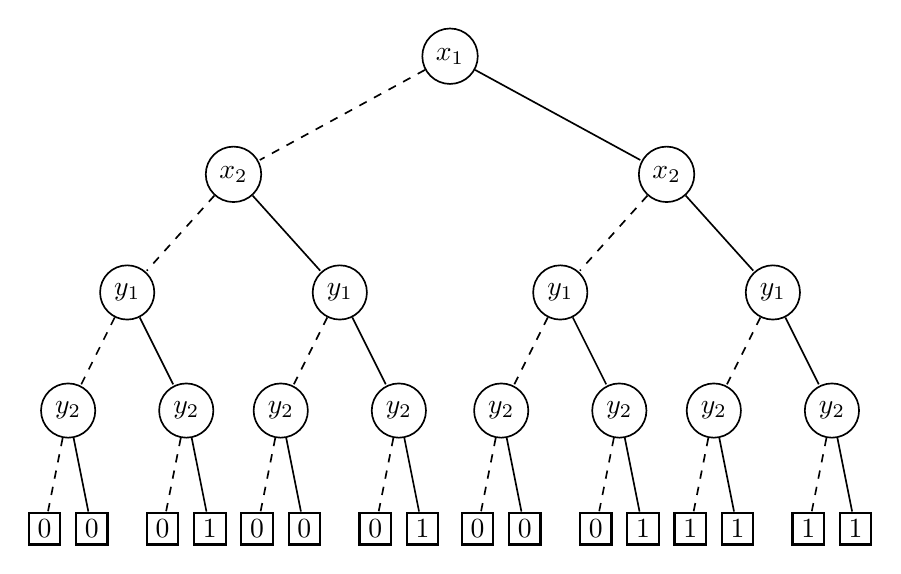
\begin{tikzpicture}[
  level 1/.style={sibling distance=55mm},
  level 2/.style={sibling distance=27mm},
  level 3/.style={sibling distance=15mm},
  level 4/.style={sibling distance=6mm},
  -,>=stealth',shorten >=0.5pt,auto,node distance=1cm,semithick,term/.style={draw,rectangle,minimum size=4mm,inner sep=0pt,outer sep=0pt,solid,thick}]
      \tikzstyle{every state}=[fill=white,draw=black,text=black,inner sep=3pt,minimum size=4pt,solid]
      
      
     \node [state] (a){$x_1$}
     child[dashed]{
      node [state] (b){$x_2$}
      child[dashed]{
	node [state] (c){$y_1$}
	child[dashed]{
	  node [state] (d){$y_2$}
	  child[dashed]{
	    node [term] (e){$0$}	    
	  }
	  child[solid]{
	    node [term] (e){$0$}	    
	  }
	}
	child[solid]{
	  node [state] (d){$y_2$}
	  child[dashed]{
	    node [term] (e){$0$}	    
	  }
	  child[solid]{
	    node [term] (e){$1$}	    
	  }
	}
      }
      child[solid]{
	node [state] (c){$y_1$}
	child[dashed]{
	  node [state] (d){$y_2$}
	  child[dashed]{
	    node [term] (e){$0$}	    
	  }
	  child[solid]{
	    node [term] (e){$0$}	    
	  }
	}
	child[solid]{
	  node [state] (d){$y_2$}
	  child[dashed]{
	    node [term] (e){$0$}	    
	  }
	  child[solid]{
	    node [term] (e){$1$}	    
	  }
	}
      }
     }
     child[solid]{
      node [state] (b){$x_2$}
      child[dashed]{
	node [state] (c){$y_1$}
	child[dashed]{
	  node [state] (d){$y_2$}
	  child[dashed]{
	    node [term] (e){$0$}	    
	  }
	  child[solid]{
	    node [term] (e){$0$}	    
	  }
	}
	child[solid]{
	  node [state] (d){$y_2$}
	  child[dashed]{
	    node [term] (e){$0$}	    
	  }
	  child[solid]{
	    node [term] (e){$1$}	    
	  }
	}
      }
      child[solid]{
	node [state] (c){$y_1$}
	child[dashed]{
	  node [state] (d){$y_2$}
	  child[dashed]{
	    node [term] (e){$1$}	    
	  }
	  child[solid]{
	    node [term] (e){$1$}	    
	  }
	}
	child[solid]{
	  node [state] (d){$y_2$}
	  child[dashed]{
	    node [term] (e){$1$}	    
	  }
	  child[solid]{
	    node [term] (e){$1$}	    
	  }
	}
      }
     };
 
  \end{tikzpicture}
  \caption{A BDT is easily derived from the truth table. Every non-terminal node is labelled with a variable and every terminal node is labelled with either 0 or 1.}
\end{figure}

\subsection*{Reduced Ordered Binary Decision Diagrams}
In order to reduce the size of the BDT we can produce a 
Binary Decision Diagram which is a reduced form of the BDT.
Making this diagram ordered over a list of variables, results in getting an Ordered Binary Decision Diagram (OBDD) which is
then unique when it is reduced until no more reduction can occur. This reduced form is called canonical form and it can be used to
extract equivalences since two different but equivalent Boolean functions always have identically structured Reduced Ordered Binary Decision Diagrams 
if they have compatible variable orderings.
\subsubsection*{Reduction Algorithm}
\noindent In order to reduce BDTs we use iteratively the rules C1-C3 until no more reductions can occur.

\begin{itemize}
\item {\bf C1:} Removal of duplicate terminals. 
\item {\bf C2:} Removal of redundant tests. 
\item {\bf C3:} Removal of duplicate non-terminals. 
\end{itemize}




\subsubsection*{ROBDD under the $[x_1,x_2,y_1,y_2]$ ordering.}

\begin{figure}[H]
  \label{fig:robdd11}
  \centering
  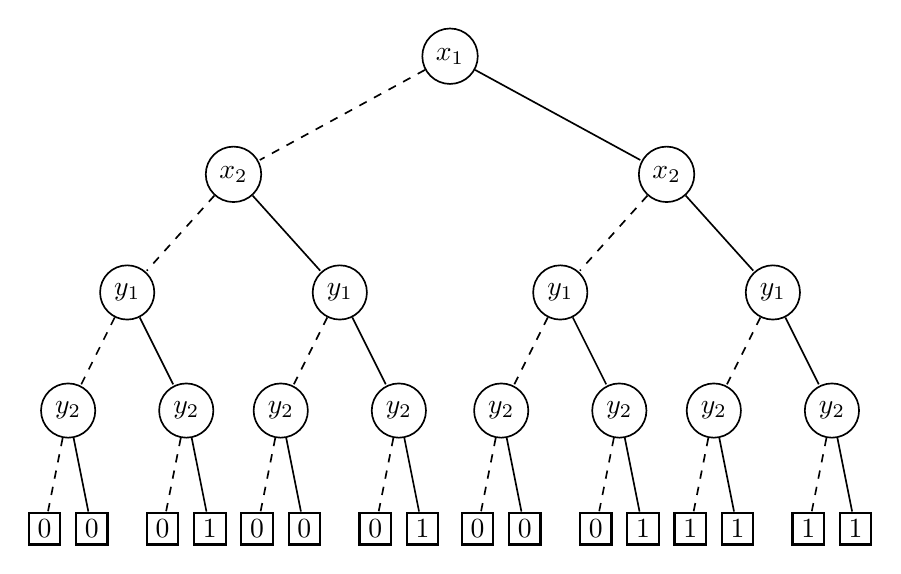
\begin{tikzpicture}[
  level 1/.style={sibling distance=55mm},
  level 2/.style={sibling distance=27mm},
  level 3/.style={sibling distance=15mm},
  level 4/.style={sibling distance=6mm},
  -,>=stealth',shorten >=0.5pt,auto,node distance=1cm,semithick,term/.style={draw,rectangle,minimum size=4mm,inner sep=0pt,outer sep=0pt,solid,thick}]
      \tikzstyle{every state}=[fill=white,draw=black,text=black,inner sep=3pt,minimum size=4pt,solid]
      
      
     \node [state] (a){$x_1$}
     child[dashed]{
      node [state] (b){$x_2$}
      child[dashed]{
	node [state] (c){$y_1$}
	child[dashed]{
	  node [state] (d){$y_2$}
	  child[dashed]{
	    node [term] (e){$0$}	    
	  }
	  child[solid]{
	    node [term] (e){$0$}	    
	  }
	}
	child[solid]{
	  node [state] (d){$y_2$}
	  child[dashed]{
	    node [term] (e){$0$}	    
	  }
	  child[solid]{
	    node [term] (e){$1$}	    
	  }
	}
      }
      child[solid]{
	node [state] (c){$y_1$}
	child[dashed]{
	  node [state] (d){$y_2$}
	  child[dashed]{
	    node [term] (e){$0$}	    
	  }
	  child[solid]{
	    node [term] (e){$0$}	    
	  }
	}
	child[solid]{
	  node [state] (d){$y_2$}
	  child[dashed]{
	    node [term] (e){$0$}	    
	  }
	  child[solid]{
	    node [term] (e){$1$}	    
	  }
	}
      }
     }
     child[solid]{
      node [state] (b){$x_2$}
      child[dashed]{
	node [state] (c){$y_1$}
	child[dashed]{
	  node [state] (d){$y_2$}
	  child[dashed]{
	    node [term] (e){$0$}	    
	  }
	  child[solid]{
	    node [term] (e){$0$}	    
	  }
	}
	child[solid]{
	  node [state] (d){$y_2$}
	  child[dashed]{
	    node [term] (e){$0$}	    
	  }
	  child[solid]{
	    node [term] (e){$1$}	    
	  }
	}
      }
      child[solid]{
	node [state] (c){$y_1$}
	child[dashed]{
	  node [state] (d){$y_2$}
	  child[dashed]{
	    node [term] (e){$1$}	    
	  }
	  child[solid]{
	    node [term] (e){$1$}	    
	  }
	}
	child[solid]{
	  node [state] (d){$y_2$}
	  child[dashed]{
	    node [term] (e){$1$}	    
	  }
	  child[solid]{
	    node [term] (e){$1$}	    
	  }
	}
      }
     };
 
  \end{tikzpicture}
  \caption{We start with the BDT over our ordering.}
\end{figure}


\begin{figure}[H]
  \label{fig:robdd12}
  \centering
  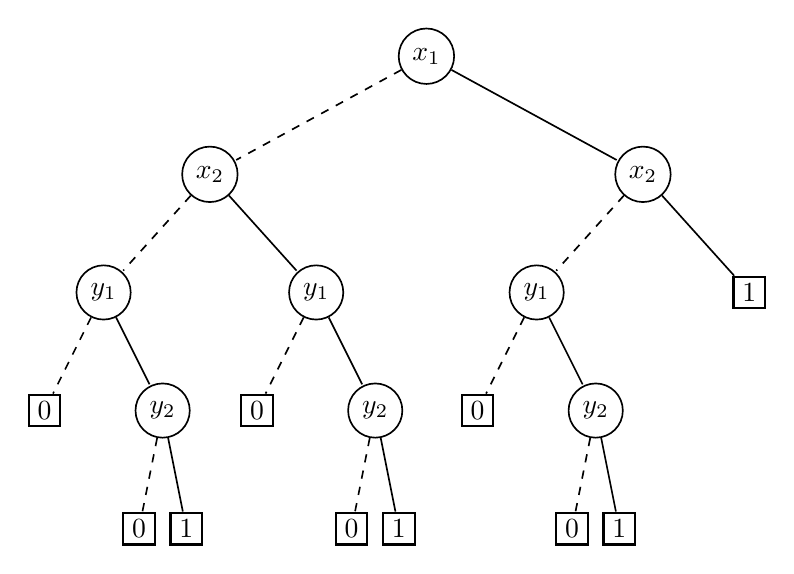
\begin{tikzpicture}[
  level 1/.style={sibling distance=55mm},
  level 2/.style={sibling distance=27mm},
  level 3/.style={sibling distance=15mm},
  level 4/.style={sibling distance=6mm},
  -,>=stealth',shorten >=0.5pt,auto,node distance=1cm,semithick,term/.style={draw,rectangle,minimum size=4mm,inner sep=0pt,outer sep=0pt,solid,thick}]
      \tikzstyle{every state}=[fill=white,draw=black,text=black,inner sep=3pt,minimum size=4pt,solid]
      
      
     \node [state] (a){$x_1$}
     child[dashed]{
      node [state] (b){$x_2$}
      child[dashed]{
	node [state] (c){$y_1$}
	child[dashed]{
	  node [term] (d){$0$}
	}
	child[solid]{
	  node [state] (d){$y_2$}
	  child[dashed]{
	    node [term] (e){$0$}	    
	  }
	  child[solid]{
	    node [term] (e){$1$}	    
	  }
	}
      }
      child[solid]{
	node [state] (c){$y_1$}
	child[dashed]{
	  node [term] (d){$0$}
	 }
	child[solid]{
	  node [state] (d){$y_2$}
	  child[dashed]{
	    node [term] (e){$0$}	    
	  }
	  child[solid]{
	    node [term] (e){$1$}	    
	  }
	}
      }
     }
     child[solid]{
      node [state] (b){$x_2$}
      child[dashed]{
	node [state] (c){$y_1$}
	child[dashed]{
	  node [term] (d){$0$}	  
	}
	child[solid]{
	  node [state] (d){$y_2$}
	  child[dashed]{
	    node [term] (e){$0$}	    
	  }
	  child[solid]{
	    node [term] (e){$1$}	    
	  }
	}
      }
      child[solid]{
	node [term] (c){$1$}
      }
     };
 
  \end{tikzpicture}
  \caption{Using C2 we remove the redundant tests and eliminate the nodes leading to them. We derive the above reduced diagram.}
\end{figure}


\begin{figure}[H]
  \label{fig:robdd1}
  \centering
  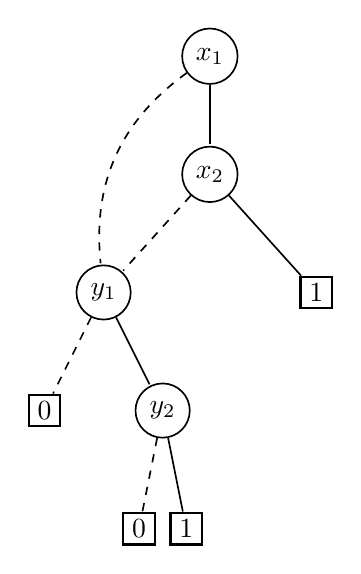
\begin{tikzpicture}[
  level 1/.style={sibling distance=55mm},
  level 2/.style={sibling distance=27mm},
  level 3/.style={sibling distance=15mm},
  level 4/.style={sibling distance=6mm},
  -,>=stealth',shorten >=0.5pt,auto,node distance=1cm,semithick,term/.style={draw,rectangle,minimum size=4mm,inner sep=0pt,outer sep=0pt,solid,thick}]
      \tikzstyle{every state}=[fill=white,draw=black,text=black,inner sep=3pt,minimum size=4pt,solid]
      
      
     \node [state] (A){$x_1$}
     
     child[solid]{
      node [state] (B){$x_2$}
      child[dashed]{
	node [state] (C1){$y_1$}
	child[dashed]{
	  node [term] (D1){$0$}	  
	}
	child[solid]{
	  node [state] (D2){$y_2$}
	  child[dashed]{
	    node [term] (E1){$0$}	    
	  }
	  child[solid]{
	    node [term] (E2){$1$}	    
	  }
	}
      }
      child[solid]{
	node [term] (C2){$1$}
      }
     };
     
     \path 
	(A) edge[dashed,bend right]			node{} (C1);
	
 
  \end{tikzpicture}
  \caption{Using C3 we remove the duplicate non-terminals, redirect the incoming edges and derive the above reduced diagram.}
\end{figure}


\begin{figure}[H]
  \label{fig:robdd13}
  \centering
  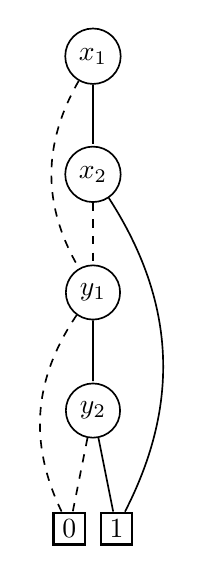
\begin{tikzpicture}[
  level 1/.style={sibling distance=55mm},
  level 2/.style={sibling distance=27mm},
  level 3/.style={sibling distance=15mm},
  level 4/.style={sibling distance=6mm},
  -,>=stealth',shorten >=0.5pt,auto,node distance=1cm,semithick,term/.style={draw,rectangle,minimum size=4mm,inner sep=0pt,outer sep=0pt,solid,thick}]
      \tikzstyle{every state}=[fill=white,draw=black,text=black,inner sep=3pt,minimum size=4pt,solid]
      
      
     \node [state] (A){$x_1$}
     
     child[solid]{
      node [state] (B){$x_2$}
      child[dashed]{
	node [state] (C1){$y_1$}
	child[solid]{
	  node [state] (D2){$y_2$}
	  child[dashed]{
	    node [term] (E1){$0$}	    
	  }
	  child[solid]{
	    node [term] (E2){$1$}	    
	  }
	}
      }
     };
     
     \path 
	(A) edge[dashed,bend right]			node{} (C1)
	(B) edge[bend left]			node{} (E2)
	(C1) edge[dashed,bend right]			node{} (E1);

 
  \end{tikzpicture}
  \caption{Using C1 we remove all the duplicate terminals. This OBDD cannot be reduced any further so we can now call it the canonical of the previous diagrams.}
\end{figure}

\subsubsection*{ROBDD under the $[x_1,y_1,y_2,x_2]$ ordering.}

\begin{figure}[H]
  \label{fig:robdd21}
  \centering
  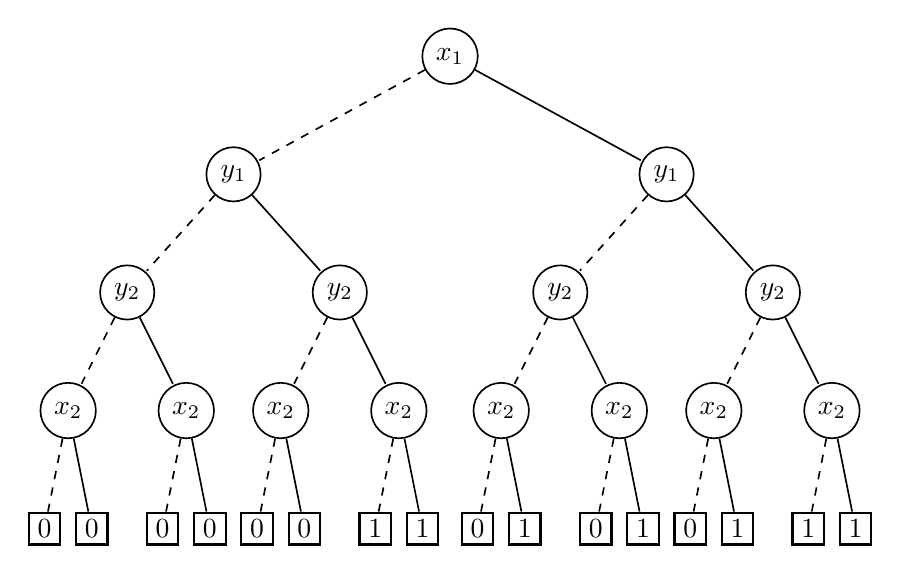
\begin{tikzpicture}[
  level 1/.style={sibling distance=55mm},
  level 2/.style={sibling distance=27mm},
  level 3/.style={sibling distance=15mm},
  level 4/.style={sibling distance=6mm},
  -,>=stealth',shorten >=0.5pt,auto,node distance=1cm,semithick,term/.style={draw,rectangle,minimum size=4mm,inner sep=0pt,outer sep=0pt,solid,thick}]
      \tikzstyle{every state}=[fill=white,draw=black,text=black,inner sep=3pt,minimum size=4pt,solid]
      
      
     \node [state] (a){$x_1$}
     child[dashed]{
      node [state] (b){$y_1$}
      child[dashed]{
	node [state] (c){$y_2$}
	child[dashed]{
	  node [state] (d){$x_2$}
	  child[dashed]{
	    node [term] (e){$0$}	    
	  }
	  child[solid]{
	    node [term] (e){$0$}	    
	  }
	}
	child[solid]{
	  node [state] (d){$x_2$}
	  child[dashed]{
	    node [term] (e){$0$}	    
	  }
	  child[solid]{
	    node [term] (e){$0$}	    
	  }
	}
      }
      child[solid]{
	node [state] (c){$y_2$}
	child[dashed]{
	  node [state] (d){$x_2$}
	  child[dashed]{
	    node [term] (e){$0$}	    
	  }
	  child[solid]{
	    node [term] (e){$0$}	    
	  }
	}
	child[solid]{
	  node [state] (d){$x_2$}
	  child[dashed]{
	    node [term] (e){$1$}	    
	  }
	  child[solid]{
	    node [term] (e){$1$}	    
	  }
	}
      }
     }
     child[solid]{
      node [state] (b){$y_1$}
      child[dashed]{
	node [state] (c){$y_2$}
	child[dashed]{
	  node [state] (d){$x_2$}
	  child[dashed]{
	    node [term] (e){$0$}	    
	  }
	  child[solid]{
	    node [term] (e){$1$}	    
	  }
	}
	child[solid]{
	  node [state] (d){$x_2$}
	  child[dashed]{
	    node [term] (e){$0$}	    
	  }
	  child[solid]{
	    node [term] (e){$1$}	    
	  }
	}
      }
      child[solid]{
	node [state] (c){$y_2$}
	child[dashed]{
	  node [state] (d){$x_2$}
	  child[dashed]{
	    node [term] (e){$0$}	    
	  }
	  child[solid]{
	    node [term] (e){$1$}	    
	  }
	}
	child[solid]{
	  node [state] (d){$x_2$}
	  child[dashed]{
	    node [term] (e){$1$}	    
	  }
	  child[solid]{
	    node [term] (e){$1$}	    
	  }
	}
      }
     };
 
  \end{tikzpicture}
  \caption{We start with the BDT over our ordering.}
\end{figure}

\begin{figure}[H]
  \label{fig:robdd22}
  \centering
  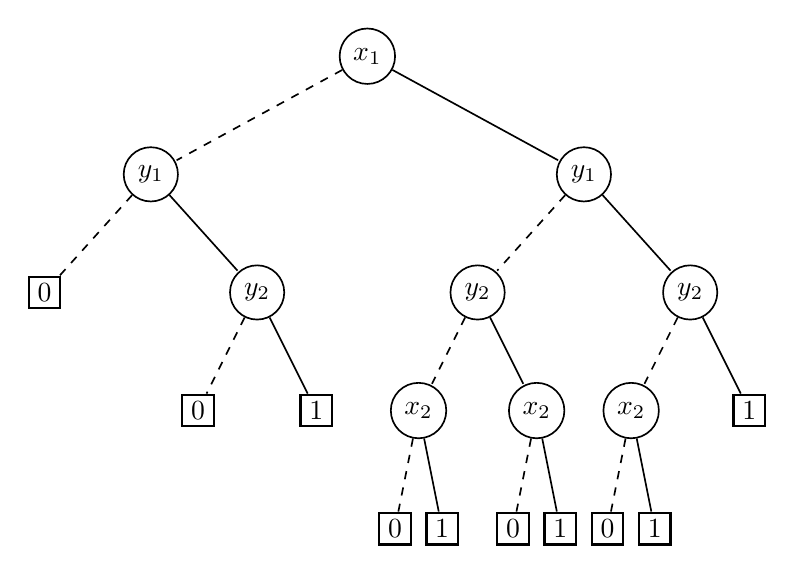
\begin{tikzpicture}[
  level 1/.style={sibling distance=55mm},
  level 2/.style={sibling distance=27mm},
  level 3/.style={sibling distance=15mm},
  level 4/.style={sibling distance=6mm},
  -,>=stealth',shorten >=0.5pt,auto,node distance=1cm,semithick,term/.style={draw,rectangle,minimum size=4mm,inner sep=0pt,outer sep=0pt,solid,thick}]
      \tikzstyle{every state}=[fill=white,draw=black,text=black,inner sep=3pt,minimum size=4pt,solid]
      
      
     \node [state] (a){$x_1$}
     child[dashed]{
      node [state] (b){$y_1$}
      child[dashed]{
	node [term] (c){$0$}
      }
      child[solid]{
	node [state] (c){$y_2$}
	child[dashed]{
	  node [term] (d){$0$}	  
	}
	child[solid]{
	  node [term] (d){$1$}
	}
      }
     }
     child[solid]{
      node [state] (b){$y_1$}
      child[dashed]{
	node [state] (c){$y_2$}
	child[dashed]{
	  node [state] (d){$x_2$}
	  child[dashed]{
	    node [term] (e){$0$}	    
	  }
	  child[solid]{
	    node [term] (e){$1$}	    
	  }
	}
	child[solid]{
	  node [state] (d){$x_2$}
	  child[dashed]{
	    node [term] (e){$0$}	    
	  }
	  child[solid]{
	    node [term] (e){$1$}	    
	  }
	}
      }
      child[solid]{
	node [state] (c){$y_2$}
	child[dashed]{
	  node [state] (d){$x_2$}
	  child[dashed]{
	    node [term] (e){$0$}	    
	  }
	  child[solid]{
	    node [term] (e){$1$}	    
	  }
	}
	child[solid]{
	  node [term] (d){$1$}	  
	}
      }
     };
 
  \end{tikzpicture}
  \caption{Using C2 we remove the redundant tests and eliminate the nodes leading to them. We derive the above reduced diagram.}

\end{figure}

\begin{figure}[H]
  \label{fig:robdd23}
  \centering
  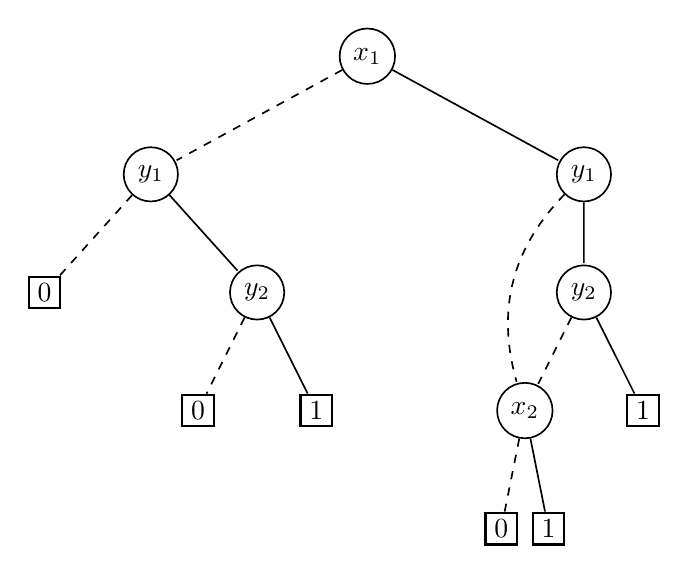
\begin{tikzpicture}[
  level 1/.style={sibling distance=55mm},
  level 2/.style={sibling distance=27mm},
  level 3/.style={sibling distance=15mm},
  level 4/.style={sibling distance=6mm},
  -,>=stealth',shorten >=0.5pt,auto,node distance=1cm,semithick,term/.style={draw,rectangle,minimum size=4mm,inner sep=0pt,outer sep=0pt,solid,thick}]
      \tikzstyle{every state}=[fill=white,draw=black,text=black,inner sep=3pt,minimum size=4pt,solid]
      
      
     \node [state] (A){$x_1$}
     child[dashed]{
      node [state] (B1){$y_1$}
      child[dashed]{
	node [term] (C1){$0$}
      }
      child[solid]{
	node [state] (C2){$y_2$}
	child[dashed]{
	  node [term] (D1){$0$}	  
	}
	child[solid]{
	  node [term] (D2){$1$}
	}
      }
     }
     child[solid]{
      node [state] (B2){$y_1$}
      child[solid]{
	node [state] (C3){$y_2$}
	child[dashed]{
	  node [state] (D5){$x_2$}
	  child[dashed]{
	    node [term] (E5){$0$}	    
	  }
	  child[solid]{
	    node [term] (E6){$1$}	    
	  }
	}
	child[solid]{
	  node [term] (D6){$1$}	  
	}
      }
     };
     
       \path 
	(B2) edge[dashed,bend right]			node{} (D5);

 
  \end{tikzpicture}
  \caption{Using C3 we remove the duplicate non-terminals, redirect the incoming edges and derive the above reduced diagram.}

\end{figure}
\begin{figure}[H]
  \label{fig:robdd24}
  \centering
  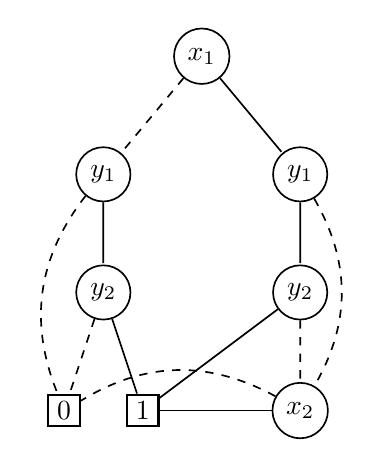
\begin{tikzpicture}[
  level 1/.style={sibling distance=25mm},
  level 2/.style={sibling distance=27mm},
  level 3/.style={sibling distance=10mm},
  level 4/.style={sibling distance=6mm},
  -,>=stealth',shorten >=0.5pt,auto,node distance=1cm,semithick,term/.style={draw,rectangle,minimum size=4mm,inner sep=0pt,outer sep=0pt,solid,thick}]
      \tikzstyle{every state}=[fill=white,draw=black,text=black,inner sep=3pt,minimum size=4pt,solid]
      
      
     \node [state] (A){$x_1$}
     child[dashed]{
      node [state] (B1){$y_1$}
      child[solid]{
	node [state] (C2){$y_2$}
	child[dashed]{
	  node [term] (D1){$0$}	  
	}
	child[solid]{
	  node [term] (D2){$1$}
	}
      }
     }
     child[solid]{
      node [state] (B2){$y_1$}
      child[solid]{
	node [state] (C3){$y_2$}
	child[dashed]{
	  node [state] (D5){$x_2$}
	  }
      }
     };
     
       \path 
       	(B1) edge[dashed,bend right]			node{} (D1)
       	(C3) edge[right]				node{} (D2)
       	(D5) edge[dashed,bend right]			node{} (D1)
       	(D5) edge[left]				node{} (D2)
	(B2) edge[dashed,bend left]			node{} (D5);

 
  \end{tikzpicture}

\caption{Using C1 we remove all the duplicate terminals. This OBDD cannot be reduced any further so we can now call it the canonical of the previous diagrams.}

\end{figure}

\subsection*{How ordering impacts the ROBDD size.}
The chosen variable ordering can have a very significant impact on the size of the ROBDD as we can see from the above. The OBDDs' 
size tend to be very sensitive to the chosen ordering. 
This however is not always the case and if we consider the OBDDs representing functions such as the parity functions and in principle
the functions that are themselves independent of the order of the variables (symmetric boolean functions), it is clear that any change 
in the ordering leaves the size of the ROBDD unaffected. \\[0.25cm]
In general however, the chosen ordering will have a significant impact to the size. If we consider the boolean function:
$(x_1 \vee x_2) \wedge (x_3 \vee x_4) \wedge ... \wedge (x_{2n-1} \vee x_{2n})$, choosing the ordering $(x_1,x_2,...x_{2n-1},x_{2n})$ will
have produce a ROBDD with 2n+2 nodes while choosing an ordering us $(x_1,x_3,...,x_{2n-1},x2,x_4,...x_{2n})$ will produce an ROBDD of $2^{n+1}$.
The level at which the result of the formula depends on a variable along with repetition, precedence and many other factors will affect the importance of the ordering.



\subsection*{An algorithm for choosing ordering}
The problem of choosing the variable ordering to produce an ROBDD of minimum size is similar to the Travelling Salesman Problem of finding the minimum path 
but propably much harder to be pictured and reason about it. Finding the minimum size is only guaranteed when comparing the resulting ROBDD of every ordering 
from the $n!$ possible permutations and it is NP-complete. The same goes for finding good or ''better''  ordering instead of the best. THis hoever can be done 
using heuristics in a less expensive manner.\\[0.25cm]
One way is by simplifying our formula using equivalences and factorisation to eliminate repetition. We can then examine and find dependancy chains. The more 
dependent the result of a formula, the higher ordering the variable should have. Another way to be considered is the use of a hill climbing procedure which will
redorder the given ordering such as the size decreases. A similar approach can be achieved by shifting the variables one by one until a minimum is reached. \\[0.25cm]
None of these methods can however guarantee a ''minimum'' size but only a better one.

\end{document}
